\documentclass{standalone}
\usepackage{tikz}
\usetikzlibrary{shapes.geometric}
\begin{document}
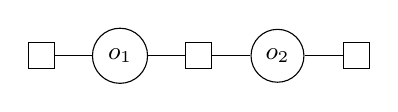
\begin{tikzpicture}[square/.style={regular polygon,regular polygon sides=4}]
    \node at (0, 0) [circle, minimum size = 0.7cm, draw] (o1) {\small $o_1$}; 
    \node at (-1, 0) [square, draw] (s_1) {};
    \node at (1, 0) [square, draw] (e_1) {};
    \node at (2, 0) [circle, draw] (o2) {\small $o_2$};
    \node at (3, 0) [square, draw] (e_2) {};

    \draw (s_1.east) -- (o1.west); 
    \draw (o1.east) -- (e_1.west);
    \draw (e_1.east) -- (o2.west);
    \draw (o2.east) -- (e_2.west);

\end{tikzpicture}
\end{document}

